\documentclass[11pt,fleqn]{article}
\usepackage{../cs188,latexsym,epsf, amsmath,amsfonts,graphicx,url}
\lecture{8}
\def\title{Note \the\lecturenumber}
\begin{document}
\maketitle


\iffalse
\documentclass[11pt,fleqn]{article}
\usepackage{latexsym,epsf,amsmath,amsfonts,graphicx,url}

\title{Note 8}

\newcommand{\F}{\mathbb{F}}
\newcommand{\Z}{\mathbb{Z}}
\newcommand{\Q}{\mathbb{Q}}
\newcommand{\R}{\mathbb{R}}
\newcommand{\C}{\mathbb{C}}

\begin{document}

\maketitle
\fi


We have developed our techniques for probabilistic reasoning in the context of \textit{static} world, in which each random variable takes a single fixed value. For example, when probing the cavity, we assume that whatever tooth has a cavity remains cavitary during the process of probing; when forecasting the weather, we assume that whether the forecaster says a rainy day or not the weather does not change in that day. In many real-world problems, we want to reason about a sequence of observations. As a follow-up of the previous weather example, consider the task of monitoring every day's actual weather based on the historical weather forecasts. Unlike the previous example, here the \textit{dynamic} aspects of the problem are essential since the weather changes day by day. Other examples include robot localization where robot moves in a space and we want to know the robot's current location based on a sequence of range sensor observations, speech recognition where the task is to figure out the actual words people say based on a segment of rapidly changing acoustic signals, etc. 

\section{Markov Model}
Markov chain (MC) is a common model to capture the dynamics of the problem. MC can be considered as a special Bayes' net where each node corresponds to the state in a given time step.

\begin{center}	
	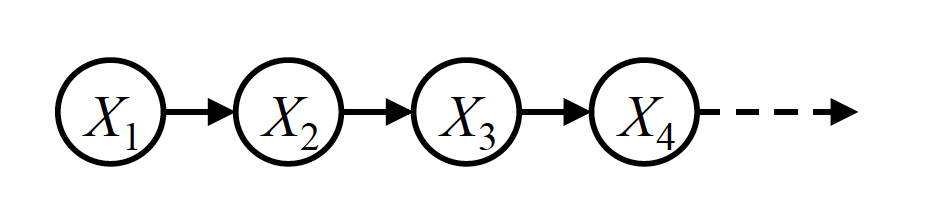
\includegraphics[width=10cm]{img/mc}
\end{center} 

MC makes the assumption that the state at each time step depends only on the previous state. In other words, given the current state $X_t$, the future state $X_{t+1}$ is conditionally independent of the entire past states $X_{t-1},\cdots,X_1$,
\begin{align}
P(X_{t+1}|X_1,\cdots,X_t) = P(X_{t+1}|X_t)
\end{align}
$P(X_{t+1}|X_t)$ is called transition model or transition probability in the MC. Another assumption that we will make on the MC throughout the course is the \textit{stationary} assumption, which states that the transition probability does not change over time, i.e.,
\begin{align}
P(X_{t+1}|X_t) = P(X_t|X_{t-1}) = \cdots
\end{align}
To fully characterize the MC, we only need a CPT for the transition model and a CPT for the probability distribution of the initial state $P(X_1)$. Once we have these two CPTs, we can represent the joint probability distribution of all states in the MC and can perform various kinds of inference tasks thereafter. 

There is a inference task that is of particular interest in the MC - the probability distribution of the state at a given time step, i.e., $P(X_t)$. For example, $X_t$ is the weather (rain/sun) in day $t$. $P(X_t)$ is the chances of the weather being rainy and sunny, respectively. By simply using the probability law on marginalization and chain rule, we can derive an iterative algorithm to calculate $P(X_t)$ as follows,
\begin{align}
\label{eqn:mini_forward}
P(x_t)&= \sum_{x_{t-1}}P(x_t,x_{t-1})\nonumber\\
&= \sum_{x_{t-1}} P(x_t|x_{t-1})P(x_{t-1})
\end{align}
Since we know the probability distribution of the initial state $P(x_1)$ and transition model $P(x_t|x_{t-1})$, we can solve $P(x_t)$ for $t=2,3,\cdots$ using (\ref{eqn:mini_forward}). This iterative procedure is called Mini-Forward algorithm.

A interesting phenomenon regarding $P(X_t)$ for a stationary MC is that as $t$ goes to infinity, $P(X_t)$ converges to a fixed probability distribution (you can think of it as a fixed probability table) whatever probability distribution the initial state has. To derive what distribution $P(X_t)$ converges to, we can use Mini-Forward algorithm,
\begin{align}
\label{eqn:stat_dist}
P(x_{\infty+1}) &= \sum_{x_{\infty}}P(x_{\infty+1},x_{\infty})\nonumber\\
&= \sum_{x_{\infty}} \underbrace{P(x_{\infty+1}|x_{\infty})}_{\text{transition probability}}P(x_{\infty})
\end{align}
In addition, we know that the probability should be summed up to one, i.e.,
\begin{align}
\label{eqn:one}
\sum_{x_\infty} P(x_\infty)=1
\end{align}
Note that (\ref{eqn:stat_dist}) and (\ref{eqn:one}) provide a system of linear equations with respect to $P(x_\infty)$. Treating the convergence distribution $P(x_\infty)$ as unknown variables, we can solve it from (\ref{eqn:stat_dist}) and (\ref{eqn:one}). $P(x_\infty)$ is called stationary distribution of the MC, and (\ref{eqn:stat_dist}) and (\ref{eqn:one}) give a bunch of conditions that the stationary distribution should satisfy.


\section{Hidden Markov Model}
As aforementioned, in many real-world problems we cannot directly gather evidence on the exact state but some noisy observations related to the actual state. Say, in the robot localization problem, we can only observe a sequence of noisy range sensor readings and hope to infer the actual location of the robot based on the sensor measurements. In this problem, the actual robot location is the hidden state variable (something we would like to know but not observable), the sensor measurements are evidence/observation variables (something we can directly observe). The model for this kind of problem is hidden Markov model.

Hidden Markov model consists of state variables that ev

\begin{center}	
	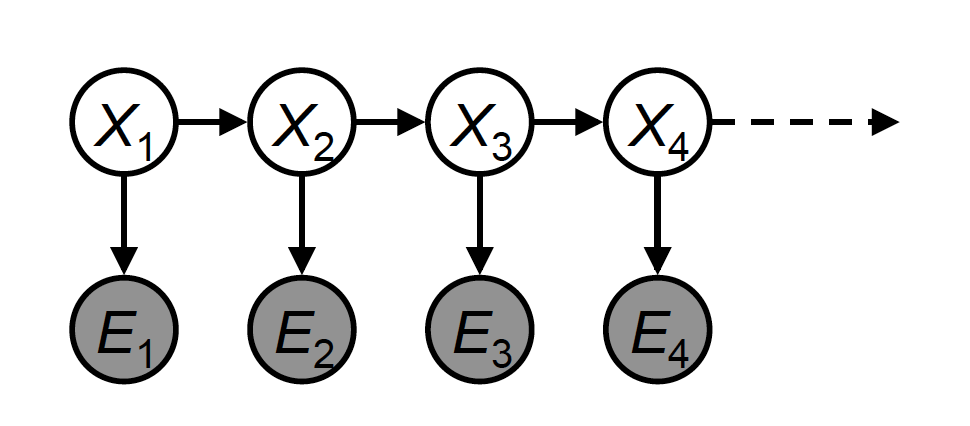
\includegraphics[width=10cm]{img/hmc}
\end{center}





\end{document}
